%%%%%%%%%%%%%%%%%%%%%%%%%%%%%%%%%%%%%%%%%
% Short Sectioned Assignment
% LaTeX Template
% Version 1.0 (5/5/12)
%
% This template has been downloaded from:
% http://www.LaTeXTemplates.com
%
% Original author:
% Frits Wenneker (http://www.howtotex.com)
%
% License:
% CC BY-NC-SA 3.0 (http://creativecommons.org/licenses/by-nc-sa/3.0/)
%
%%%%%%%%%%%%%%%%%%%%%%%%%%%%%%%%%%%%%%%%%

%----------------------------------------------------------------------------------------
%	PACKAGES AND OTHER DOCUMENT CONFIGURATIONS
%----------------------------------------------------------------------------------------

\documentclass[paper=a4, fontsize=11pt]{scrartcl} % A4 paper and 11pt font size

\usepackage[T1]{fontenc} % Use 8-bit encoding that has 256 glyphs
\usepackage{fourier} % Use the Adobe Utopia font for the document - comment this line to return to the LaTeX default
\usepackage[english]{babel} % English language/hyphenation
\usepackage{amsmath,amsfonts,amsthm} % Math packages

\usepackage{lipsum} % Used for inserting dummy 'Lorem ipsum' text into the template

\usepackage{sectsty} % Allows customizing section commands
\allsectionsfont{\centering \normalfont\scshape} % Make all sections centered, the default font and small caps

\usepackage{fancyhdr} % Custom headers and footers

% my packages
\usepackage{commath}
\usepackage{mathtools}
\usepackage{graphicx}
\usepackage{algorithm}
\usepackage[]{algpseudocode}
\DeclarePairedDelimiter{\ceil}{\lceil}{\rceil}
\usepackage{tikz}
\usepackage{pgfplots}
\pgfplotsset{compat=newest}
\usetikzlibrary{shapes.geometric,arrows,fit,matrix,positioning}
\tikzset
{
    treenode/.style = {white, circle, draw=black, fill=black, align=center, minimum size=1cm},
    nvnode/.style = {circle, draw=black, align=center, minimum size=1cm},
    optnode/.style = {circle, draw=red, red, align=center, minimum size=1cm},
    subtree/.style  = {isosceles triangle, draw=black, align=center, minimum height=0.5cm, minimum width=1cm, shape border rotate=90, anchor=north}
}

\usepackage{hyperref}

\pagestyle{fancyplain} % Makes all pages in the document conform to the custom headers and footers
\fancyhead{} % No page header - if you want one, create it in the same way as the footers below
\fancyfoot[L]{} % Empty left footer
\fancyfoot[C]{} % Empty center footer
\fancyfoot[R]{\thepage} % Page numbering for right footer
\renewcommand{\headrulewidth}{0pt} % Remove header underlines
\renewcommand{\footrulewidth}{0pt} % Remove footer underlines
\setlength{\headheight}{13.6pt} % Customize the height of the header

\numberwithin{equation}{section} % Number equations within sections (i.e. 1.1, 1.2, 2.1, 2.2 instead of 1, 2, 3, 4)
\numberwithin{figure}{section} % Number figures within sections (i.e. 1.1, 1.2, 2.1, 2.2 instead of 1, 2, 3, 4)
\numberwithin{table}{section} % Number tables within sections (i.e. 1.1, 1.2, 2.1, 2.2 instead of 1, 2, 3, 4)

\setlength\parindent{0pt} % Removes all indentation from paragraphs - comment this line for an assignment with lots of text

% new commands
\newcommand{\filename}[1]{\textbf{\textit{#1}}}
\newcommand{\funcname}[1]{\textbf{#1}}
\newcommand{\inv}{^{\raisebox{.2ex}{$\scriptscriptstyle-1$}}}
\renewcommand{\vec}[1]{\mathbf{#1}}

\makeatletter
\renewcommand*\env@matrix[1][*\c@MaxMatrixCols c]{%
  \hskip -\arraycolsep
  \let\@ifnextchar\new@ifnextchar
  \array{#1}}
\makeatother

\makeatletter
\def\BState{\State\hskip-\ALG@thistlm}
\makeatother

\DeclareMathOperator*{\argmin}{arg\,min} % Jan Hlavacek

%----------------------------------------------------------------------------------------
%	TITLE SECTION
%----------------------------------------------------------------------------------------

\newcommand{\horrule}[1]{\rule{\linewidth}{#1}} % Create horizontal rule command with 1 argument of height

\title{	
\normalfont \normalsize 
\textsc{Mathematical foundations of computer graphics and vision} \\ [25pt] % Your university, school and/or department name(s)
\horrule{0.5pt} \\[0.4cm] % Thin top horizontal rule
\huge Exercise 3. MLS For Curves, Meshes and Images\\ % The assignment title
\horrule{2pt} \\[0.5cm] % Thick bottom horizontal rule
}

\author{Dongho Kang \\ \small 16-948-598} % Your name

\date{\normalsize April 2, 2017} % Today's date or a custom date

\begin{document}

\maketitle % Print the title

%----------------------------------------------------------------------------------------
%	README
%----------------------------------------------------------------------------------------

MATLAB R2016b version was used for coding and testing:

\begin{center}
MathWorks, MATLAB R2016b (9.1.0.441655) \\
64-bit (maci64) 
\end{center}

The \filename{code} directory contains followings:

\begin{itemize}
	\item \filename{main.m} \quad Script .m file for exercise.
	\item \filename{functions dir} \quad Function .m files 
		\begin{itemize}
			\item \funcname{SolveWithLP} \quad Function .m file for solving a problem with the LP and simple testing.
			\item \funcname{SplitProblem} \quad Function .m file for split a parent problem into two children problems.
			\item \funcname{FindBestCandidate} \quad Function .m file for finding the best candidate between two children node.
			\item \funcname{PushToStack} \quad Function .m file for stack push operation.
			\item \funcname{PopFromStack} \quad Function .m file for stack pop operation.
			\item \funcname{NewProblem} \quad Function .m file for creating new problem (instance of struct).    
			\item \funcname{FindInliers} \quad Function .m file for finding inliers with a input model.    
			\item and other sub-functions: \funcname{VisualizeMatch}, \funcname{SaveOptHistory}, \funcname{ComputeInlierLb}
		\end{itemize}
	\item \filename{data dir} \quad data and image files provided.
\end{itemize}

For running exercise, adjust threshold parameter (default of 3 pixel) and run the \filename{main.m} on the MATLAB environment. More details are stated in the \textit{Running} section.

%----------------------------------------------------------------------------------------
%	PROBLEM 1
%----------------------------------------------------------------------------------------

\section{exercise part 1: Curve and Surface Reconstruction Using MLS}

TODO
In this exercise, branch and bound algorithm based on depth-first search(DFS) was implemented. The implementation steps are as follows: 

\begin{itemize}
\item derivation of the equation of the MLS based surfaces 
\item evaluation and plotting of the derived $f(x)$
\item logging and plotting the result of branch and bound algorithm
\end{itemize}  


%----------------------------------------------------------------------------------------
%	Curve derivation
%----------------------------------------------------------------------------------------
\subsection{Curve derivation}



%----------------------------------------------------------------------------------------
%	Curves plotting
%----------------------------------------------------------------------------------------
\subsection{Curves plotting}

%----------------------------------------------------------------------------------------
\subsubsection{Description}

%----------------------------------------------------------------------------------------
\subsubsection{Running}

%----------------------------------------------------------------------------------------
\subsubsection{Result}


%----------------------------------------------------------------------------------------
%	Smoothing meshes
%----------------------------------------------------------------------------------------
\subsection{Smoothing meshes}

%----------------------------------------------------------------------------------------
\subsubsection{Description}

%----------------------------------------------------------------------------------------
\subsubsection{Running}

%----------------------------------------------------------------------------------------
\subsubsection{Result}

%----------------------------------------------------------------------------------------
%	Speeding up mesh smoothing
%----------------------------------------------------------------------------------------
\subsection{Speeding up mesh smoothing}

%----------------------------------------------------------------------------------------
\subsubsection{Description}

\url{https://github.com/jefferislab/MatlabSupport/tree/master/ann_wrapper}

%----------------------------------------------------------------------------------------
\subsubsection{Running}

%----------------------------------------------------------------------------------------
\subsubsection{Result}

%----------------------------------------------------------------------------------------
%	PROBLEM 2
%----------------------------------------------------------------------------------------

\section{exercise part 2: Image Deformation Using Moving Least Squares}


%----------------------------------------------------------------------------------------
\subsubsection{Branch and bound}

Implemented branch and bound algorithm for finding optimal solution of the consensus set maximization problem. The depth-first search based on stack data structure was used. The stack has two operation \funcname{PopFromStack} and \funcname{PushToStack}. \\

The pseudo-code of the implementation is as follows: 

\begin{algorithm}
\caption{Branch and bound}\label{euclid}
\begin{algorithmic}[1]
\State \textit{P0} $\gets$ whole problem space
\State init. $\textit{opt}$ $\gets$ variable for optimal solution (bound of inliers)
\State init. $\textit{stack}$ 
\State \textit{push(stack, P0)}
\State 
\While {\textit{stack} is not empty}
	\State \textit{Parent} = \textit{pop(stack)}
	\If {\textit{Parent.ObjUpperBound} < \textit{opt.LowerBound} } 
		\State \textbf{continue;} $\gets$ bad bound. does not contain optimum for sure
	\EndIf
	\State
	\If {$\textit{Parent.ObjLowerBound} \geq \textit{opt.LowerBound}$}
        		\State \textit{opt} = (\textit{Parent.ObjUpperBound, Parent.ObjLowerBound})
        \EndIf
        	\State
	\If {$\textit{Parent.ObjUpperBound} - \textit{Parent.ObjLowerBound} < 1$}
        		\State \textbf{continue;} $\gets$ \textit{Parent} is a leaf node thus do not split
        \EndIf
        \State
        \State (\textit{LeftChild, RightChild}) = \textit{split(Parent)}
        \State \textit{solveLP(LeftChild, RightChild)} $\gets$ solve both problems by LP and test
	\State
	\State \textit{(BetterChild, WorseChild) = findbetter(LeftChild, RightChild)}
	\State \textit{push(stack, WorseChild)}	
	\State \textit{push(stack, BetterChild)} $\gets$ \textit{BetterChild} should be on the top of stack
\EndWhile
\State
\State \textit{opt} $\gets$ now optimal solution  
\end{algorithmic}
\end{algorithm}

\pagebreak

The several criteria/strategies of implementation were defined as follows

\begin{enumerate}
\item push the original problem $P0$ to the problem stack.
\item start iteration. The iteration of branch and bound terminates when the problem stack is empty
\item bad bound check criteria: 
	\begin{itemize}
	\item $m^*$ is the highest lower bound of the number of inliers obtained so far.
	\item if the upper cardinality bound of a problem $< m^*$ then there's no optimum for sure.
	\item pop the problem from the stack without splitting.
	\end{itemize}
\item optimal solution update criteria :
	\begin{itemize}
	\item if the lower cardinality bound of a problem $lb$ is $lb \geq$ the lower cardinality bound of the optimal solution found so far, then update the optimal solution as $lb$.  
	\end{itemize}
\item convergence criteria: if the lower and upper cardinality bound are nearer than 1, stop split. 
	\begin{itemize}
	\item iteration can be terminated because the cardinality bound converged to optimum. 
	\item but here, to check whether obtained optimum is indeed global optimum, do not terminate iteration but check remaining problems by continuing depth-first search. 
	\end{itemize}
\item split the problem space and branching: splitting in half along the longest dimension. 
\item solve children problems and obtain the cardinality bound by the LP and simple test
	\begin{itemize}
	\item compute the upper bound of the number of inliers: the LP with the formulation of (1.1.1) was exploited.
	\item compute the lower bound of the number of inliers: simple test with the model $\Theta$ obtained by LP. Details are stated below.
	\end{itemize}
\item after solving children problems, push \textit{worse} child problem to the stack first, and then push \textit{better} child:
	\begin{itemize}
	\item \textit{better} child is a problem with a larger lower cardinality bound. If two children have the same lower cardinality bound, then choose one with a larger upper cardinality bound.
	\item as pushing two children, top of the stack is the \textit{better} child now. Thus the \textit{better} child will be popped in the next iteration step. 
	\item this strategy is for exploring \textit{better} problem first for reducing running time. 
	\end{itemize}
\item iteration terminates with the global optimal cardinality bound. 
\end{enumerate}

\paragraph{Solving a problem} The problem solving step is getting upper bound and lower bound of the number of inliers. Given a certain problem, solves the problem with the LP defined in (1.1.1). Then, the optimal solution of the relaxed problem $(T_{x}^*, T_{y}^*)$ and the objective cost $c^{T}\vec{x}^*$ are obtained from:

\begin{align}
\vec{x}^* &= (T_{x}^*, T_{y}^*, z_{1}^*, \dots, z_{n}^*, w_{1x}^*, \dots, w_{nx}^*, w_{1y}^*, \dots, w_{ny}^*)^{T} \\
c^{T} \vec{x}^* &= - z_{1}^* - z_{2}^* - \dots - z_{n}^*
\end{align}

The (-)objective cost, $-c^{T}\vec{x}^*$ can be set as the upper bound of inliers since the the number of inliers of that problem space never exceeds  $-c^{T}\vec{x}^*$. \\

Besides, the lower bound of inliers can be obtained by simple test with $(T_{x}^*, T_{y}^*)$ and is set as the $card(S_{I})$ as follows:

\begin{equation}
\begin{split}
card(&S_{I})  \\
s.t. 	&\quad \abs{x_{i} + T_{x}^* - x_{i}'} \leq \delta, \forall i \in S_{I} \subseteq S \\
	&\quad \abs{y_{i} + T_{y}^* - y_{i}'} \leq \delta, \forall i \in S_{I} \subseteq S
\end{split}
\end{equation}

This was implemented as the function \funcname{SolveWithLP}.

%----------------------------------------------------------------------------------------
%	RUNNING
%----------------------------------------------------------------------------------------
\subsection{Running}

Run the script \filename{main.m} after setting the parameters. 

\begin{itemize}
\item \textit{threshold} : threshold for inliers. Default is 3 (px).
\item \textit{padding} : the width of black padding between left and right image for figure(1). Default is 10 (px).
\end{itemize}

%----------------------------------------------------------------------------------------
%	RESULT
%----------------------------------------------------------------------------------------
\subsection{Result}

The optimal solution $(T_{x}^*, T_{y}^*)$ found by branch and bound for the given problem is as follows:

\begin{table}[h]
\captionof{table}{The global optimal solution obtained by branch and bound} \label{tab:title} 
\centering
\begin{tabular}{| c | c | c | }
\hline 
$T_{x}^*$		&	$T_{y}^*$		&	cardinality bound \\
\hline  
-232.00		&	-156.81		&	(15, 15.449) \\
\hline
\end{tabular}
\end{table}

Inlier indices are $(3, 8, 9, 15, 16, 20, 26, 31, 32, 34, 35, 40, 42, 45, 51)$. The identified inliers and plot of cardinality bounds are as follows. The red lines indicate outliers and the green lines indicate inliers: 

\begin{figure}[h]
\caption{The identified inlier and outlier correspondences\label{fig:simple}}
\noindent\makebox[\textwidth]{
  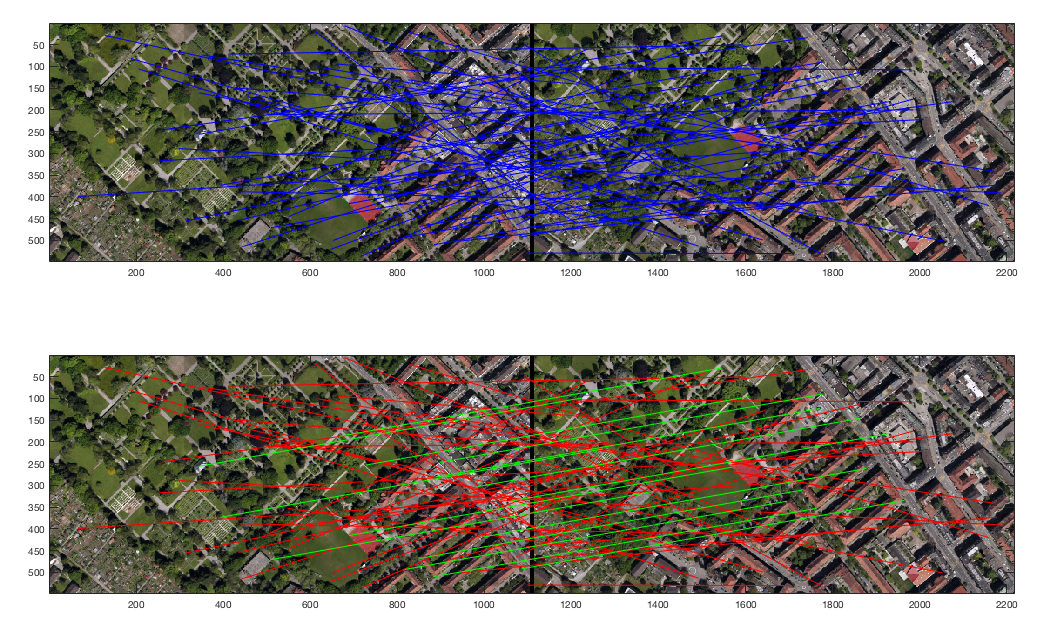
\includegraphics[width=1.0\textwidth]{inlier}
}
\end{figure} 

\begin{figure}[H]
\caption{The convergence of the cardinality bounds\label{fig:simple}}
\noindent\makebox[\textwidth]{
  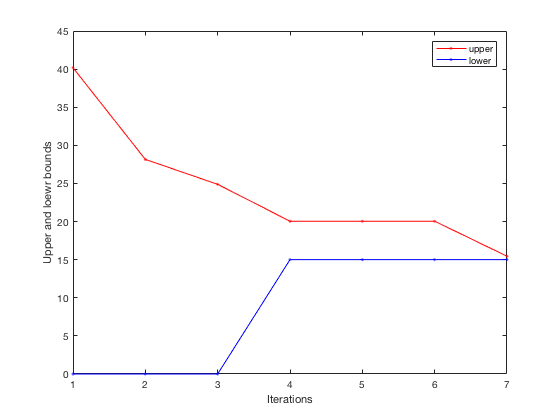
\includegraphics[width=1.0\textwidth]{cardinality_bound}
}
\end{figure} 

\pagebreak

The branch and bound iteration can be described as the following binary tree illustration:

\begin{figure}[H]
\centering
\caption{An illustration of DFS tree: one step before exploring $P11$ \label{fig:simple}}
{
    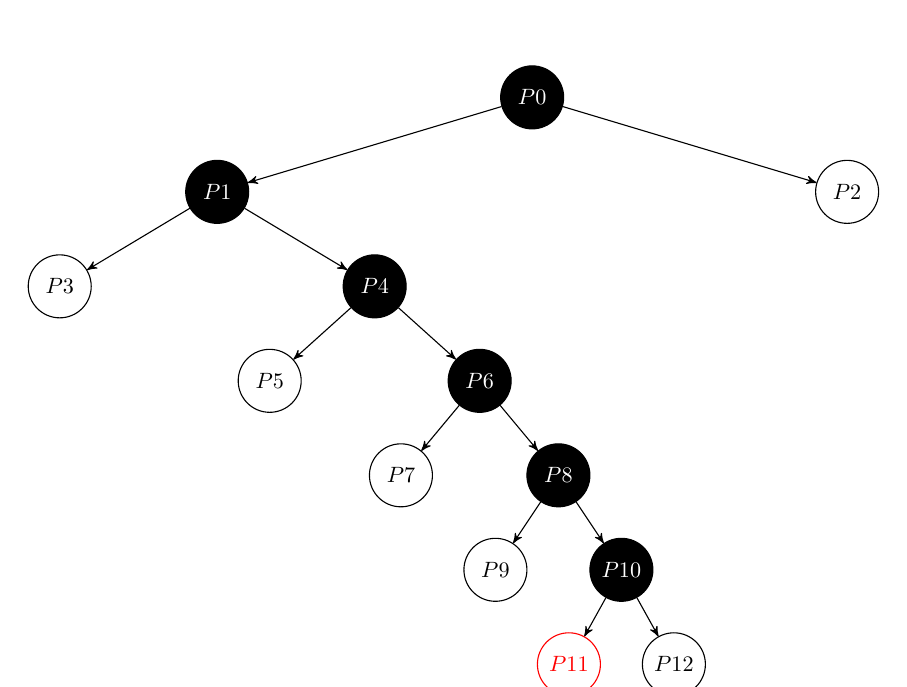
\begin{tikzpicture}[->,>=stealth', level/.style={sibling distance = 10cm/#1, level distance = 1.5cm}, scale=0.8,transform shape]
    \node [treenode] {$P0$} % (0, 40.17)
    child
    {
        node [treenode] {$P1$} %\\ (0, 28.15)} 
        child
        {
            node [nvnode] {$P3$} % \\ (0, 5.05)} 
        }
        child
        {
            node [treenode] {$P4$} % \\ (0, 24.88)}
            child 
            {
	    	node [nvnode] {$P5$} % \\ (0, 5.56)}
            }
            child 
            {
	    	node [treenode] {$P6$} % \\ (15, 20.04)}	        
		child 
            	{
	    		node [nvnode] {$P7$} % \\ (0, 2.88)}	        
            	}
		child 
            	{
	    		node [treenode] {$P8$} % \\ (0, 16.46)}	        
			child 
            		{
	    		node [nvnode] {$P9$} % \\ (0, 1.53)}	        
            		}
			child 
            		{
	        	    		node [treenode] {$P10$} %\\ (0, 15.89)}	        
        				child 
                    		{
        	    				node [optnode] {$P11$}  %\\ (15, 15.44)}	        
                    		}
				child 
                    		{
        	    				node [nvnode] {$P12$} %\\ (0, 1.37)}	        
                    		}
            		}
            	}
            }
        }
    }
    child
    {
    	node [nvnode] {$P2$} % \\ (0, 11.52)}
    }
;
% ------------------------------------------------ put the text into subtree nodes
\end{tikzpicture}
}
	\caption{An illustration of DFS stack: one step before popping $P11$ \label{fig:simple}}
	\centering
        \begin{tabular}{ | c c c c c c c }
        \hline
        P2 & P3 & P5 & P7 & P9 & P12 & P11 \\ 
        \hline
        \end{tabular} 
        
        	\caption{Problems \label{tab:title}}
	\centering
        \begin{tabular}{ | c | c | c | c | c | c |}
        \hline
         	& $\Theta_{Lb}$ 	& $\Theta_{Ub}$ 	& $\Theta_{Opt}$ 	& ObjLb & ObjUb \\ 
        \hline
        P0 & (-1104, -549)		& (1104, 549)		& (-140.94, -106.08)	& 0 & 40.17\\ 
        \hline
        P1 & (-1104, -549)		& (0, 549)			& (-336.28, -74.21)	& 0 & 28.15 \\ 
        \hline
        P2 & (0, -549) 		& (1104, 549)		& (432.47, 25.20)	& 0 & 11.52\\
        \hline
        P3  & (-1104, -549)	& (-552, 549) 		& (-665.11, -66.06)	& 0 & 5.05\\
        \hline
        P4  & (-552, -549)		& (0, 549)			& (-238.00, -154.00)	& 0 & 24.88\\
        \hline
        P5   & (-552, 0) 		& (0,549)			& (-239.45, 198.5954)	& 0 & 5.56\\ 
        \hline
        P6   & (-552, -549) 	& (-552, -549)		& (0, 0) 			& 15 & 20.04\\ 
        \hline
        P7   & (-552, -549) 	& (-276, 0) 		& (-436.00, -259.00) & 0 & 2.88\\ 
        \hline
        P8   & (-276, -549) 	& (0, 0) 			& (-232.00, -158.18)	& 0 & 16.46\\ 
        \hline
        P9   & (-276, -549) 	& (0, -275)		& (-154.00, -401.97)	& 0 & 1.53\\ 
        \hline
        P10 & (-276, -274)		& (0, 0)			& (-232.00, -156.94)	& 0 & 15.89\\
        \hline
        P11 & (-276, -274)		& (-138, 0)		& (-232.00, -156.81)	& 15 & 15.44\\
        \hline 
        P12 & (-138, -274)		& (0, 0)			& (-38.00, -99.03)	& 0 & 1.37\\
        \hline
        \end{tabular}
\end{figure}

As popping $P11$ from the stack, optimal solution is obtained but, since $P2, P3, P5, P7, P8, P12$ are still in the stack, algorithm does not terminate. However, These problems have \textit{bad bound} i.e. have smaller ObjUb (upper bound of the card.) than $P11$'s ObjLb (lower bound of the cardinality), and cannot be a optimal for sure, thus are popped without splitting and the algorithm terminates.

%----------------------------------------------------------------------------------------
%	DISCUSSION
%----------------------------------------------------------------------------------------
\subsection{Discussion}

Some comments for the bound of cardinality:

\begin{itemize}
\item The lower bound of cardinality for optimal solution monotonically increases. 
\item The upper bound of cardinality for optimal solution not necessarily monotonically decreases.
	\begin{itemize}
	\item if the first convergence (local optimal solution) is not the global optimal solution, then the upper bound of cardinality can be increased as continuing depth-first search.
	\end{itemize}
\item The global optimal solution is obtained by branch and bound algorithm. 
\end{itemize}

%===================================================================
%PART 1-3
%-------------------------------------------------------------------
%off file loading: bun.off
%calculating new V matrix...
%for sigma = 0.01
%NORMAL running time = 43.3832
%off file saving: bun_sig0.01_it10.off
%for sigma = 0.02
%NORMAL running time = 36.1822
%off file saving: bun_sig0.02_it10.off
%for sigma = 0.03
%NORMAL running time = 40.4655
%off file saving: bun_sig0.03_it10.off
%-------------------------------------------------------------------
%off file loading: bunny.off
%calculating new V matrix...
%for sigma = 0.01
%NORMAL running time = 34.6238
%off file saving: bunny_sig0.01_it10.off
%for sigma = 0.02
%NORMAL running time = 34.6699
%off file saving: bunny_sig0.02_it10.off
%for sigma = 0.03
%NORMAL running time = 35.1106
%off file saving: bunny_sig0.03_it10.off
%-------------------------------------------------------------------
%off file loading: bunny2.off
%calculating new V matrix...
%for sigma = 0.01
%NORMAL running time = 34.9052
%off file saving: bunny2_sig0.01_it10.off
%for sigma = 0.02
%NORMAL running time = 35.721
%off file saving: bunny2_sig0.02_it10.off
%for sigma = 0.03
%NORMAL running time = 36.2177
%off file saving: bunny2_sig0.03_it10.off
%-------------------------------------------------------------------
%off file loading: cat.off
%calculating new V matrix...
%for sigma = 80
%NORMAL running time = 1.3411
%off file saving: cat_sig80_it10.off
%for sigma = 90
%NORMAL running time = 1.1566
%off file saving: cat_sig90_it10.off
%for sigma = 100
%NORMAL running time = 1.1426
%off file saving: cat_sig100_it10.off
%
%
%===================================================================
%PART 1-4
%-------------------------------------------------------------------
%off file loading: bun.off
%calculating new V matrix using ANN...
%for sigma = 0.01
%ANN running time = 16.3398
%off file saving: bun_sig0.01_it10_ANN.off
%for sigma = 0.02
%ANN running time = 47.1852
%off file saving: bun_sig0.02_it10_ANN.off
%for sigma = 0.03
%ANN running time = 115.1704
%off file saving: bun_sig0.03_it10_ANN.off
%-------------------------------------------------------------------
%off file loading: bunny.off
%calculating new V matrix using ANN...
%for sigma = 0.01
%ANN running time = 12.4567
%off file saving: bunny_sig0.01_it10_ANN.off
%for sigma = 0.02
%ANN running time = 46.1488
%off file saving: bunny_sig0.02_it10_ANN.off
%for sigma = 0.03
%ANN running time = 108.848
%off file saving: bunny_sig0.03_it10_ANN.off
%-------------------------------------------------------------------
%off file loading: bunny2.off
%calculating new V matrix using ANN...
%for sigma = 0.01
%ANN running time = 15.2887
%off file saving: bunny2_sig0.01_it10_ANN.off
%for sigma = 0.02
%ANN running time = 46.4121
%off file saving: bunny2_sig0.02_it10_ANN.off
%for sigma = 0.03
%ANN running time = 129.9024
%off file saving: bunny2_sig0.03_it10_ANN.off
%-------------------------------------------------------------------
%off file loading: cat.off
%calculating new V matrix using ANN...
%for sigma = 80
%ANN running time = 1.6675
%off file saving: cat_sig80_it10_ANN.off
%for sigma = 90
%ANN running time = 1.1994
%off file saving: cat_sig90_it10_ANN.off
%for sigma = 100
%ANN running time = 1.2392
%off file saving: cat_sig100_it10_ANN.off


\end{document}